\documentclass[12pt]{article}
\usepackage[margin=1in]{geometry}
\usepackage[pdftex]{graphicx}
\usepackage{multirow}
\usepackage{setspace}
\usepackage{enumitem}
\pagestyle{plain}

\begin{document}

\noindent
% Course information
\begin{tabular*}{\textwidth}{l @{\extracolsep{\fill}} r}
  & \multirow{3}{*}{
\includegraphics[height=1.0in]{logo.jpg}} \\
  \large Intro to Physics Computation & \\
  \large Fall Quarter 2021 & \\
  \large Physics 40 & \\
\end{tabular*}
\vspace{10mm}

\noindent
% Professor information
\begin{tabular}{ l l }
  \multirow{6}{*}{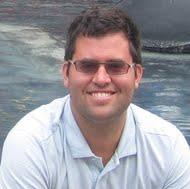
\includegraphics[height=1.25in]{mike.jpg}} & \\
  & \\
  & \large Michael Mulhearn \\
  & \large mulhearn@physics.ucdavis.edu \\
  & \large Physics 317 \\
  & \\
\end{tabular}
\vskip 0.5cm
\noindent
\textbf {Lectures:} M,W 3:10-4:00 PM in Kerr 293
\begin{tabbing}
\hspace*{3em}\= \hspace*{5em} \= \kill % set the tabbings
\textbf {Lab:}    \> Section 1: \> T,H 3:40-5:30 PM (Physics 185)
\end{tabbing}
\noindent
\textbf {Text:}\\
Online lecture notes at {\tt https://www.scipy-lectures.org}\\
Lab Manual available on course website\\
Gezerlis ``Numerical Methods in Physics with Python'' is available online at the UC Davis library.\\
% Garcia?

\noindent
\textbf{Office Hours:} Thursdays 2:30-3:30 PM \\

\noindent
\textbf{Lab Instructor:} Keerthi Vasan (kvch@ucdavis.edu) \\

\noindent
\textbf {Course Description:}  
Introduction to programming with examples from numerical analysis and
computational physics. Introduction to modern tools used for
scientific analysis and computer algebra.\\

\noindent \textbf{Lectures:} 
The primary emphasis of this course will be on learning by doing.  The
purpose of the lecture is enrichment to better prepare you for the lab
activities.  The lectures will be a mix of traditional board lecture
and projected live computing.\\

\noindent 
\textbf{Labs:} The computing labs are the essential activity
for this course.  Attendance will be taken during the first lab of
each week.  The lab activities may be finished outside of lab, but
must be posted to the course website by Friday evening in order to be
graded.  If you do not complete an assignment, submit what you were
able to finish before the deadline.\\

\noindent
\textbf{Quizzes:} Starting in Week 2, there will be a short low-stakes
quiz at the start of each Wednesday lecture.  \\

\noindent
\textbf{Interviews:} Each week I will select a subset of students for
a brief interview during the Thursday lab section. \\

\noindent \textbf{Late and Missing Evaluations:}\\ 
You should always submit whatever you have completed from the week's
lab assignments before the Friday deadline.  Each student may submit
or update one week's worth of lab assignments by the following Monday
night (Tuesday if Monday is a holiday) after the deadline, twice
during the quarter, with no penalty.  At the end of the quarter,
before the final exam, students may update one week's worth of lab
assignments which will replace their original grade.  The lowest quiz
grade will be dropped, but not if more than one quiz was excused for
another reason.  One lab absence will be excused when computing the
attendance grade.\\

\noindent
\textbf{Final Grades:} The final grades will be based on a weighted
average of the lab exercises, exams, quizzes, interviews, and lab
attendance. \\

\noindent
\textbf {Jupyter Notebooks:}\\ 
The lab manual describes numerical problems which you should complete
with Scientific Python in Jupyter Notebooks.  Even though you may work
together, each student must maintain their own notebook for each lab.
Details on preparing and submitting your notebooks to the course site
are provided in lab manual.\\

\noindent
\textbf {Pencil and Paper:}\\ 
Occassionally, the lab manual will assign pencil and paper
computations.  When requested, take a picture of your pencil and
paper computations, or scan them to PDF, and submit it to the course website along
with your Jupyter Notebook.\\


\noindent
\textbf {Reinventing the Wheel:}\\
There are many exercises in this course which involve implementing
software that is likely already available elsewhere.  This approach
is usually a bad idea.  It is a programming {\em anti-pattern} called
``Reinventing the Wheel''.  Generally one should use library functions
instead of homemade solutions whenever possible, as the library
versions are thoroughly debugged.  In this case, however, we are doing
this deliberately as an exercise.  Even when you are quite experienced
at programming, you will sometimes opt to re-implement something as a
learning experince, just as we are doing here.  The anti-pattern would
be to continue using the homebrew solution after the learning
experience, instead of using a superior existing solution.\\

\noindent
You may use the internet to search for solutions to specific technical
challenges, but you {\em may not} search for top-level solutions to
the assignments.  So ``how to use a while loop in Python'' is
perfectly fine but ``how to sum fractions in Python'' is not.  The
interviews and quizes are designed to check that you understand the
completed exercises at a level that would be difficult to reach with
cut-and-paste.\\


\newpage

\noindent \textbf{Campus Ready:}\\ 
Please review the information for students provided at:
\begin{quote}
{\tt https://campusready.ucdavis.edu/students-and-families}.\\
\end{quote}

\noindent \textbf{Daily Symptom Survey:}\\ 
You must complete the daily symptom survey and receive an ``Approved''
status to attend any in-person activities.  The instructor may spot
check your daily symptom survey, so be prepared to present it.  The
instructor may ask all attending students to forward them their daily
symptom survey on any particular day.  If your status from the daily
symptom survey prohibits attending a required in-person course activity,
forward the results to your instructor and follow the instructions
below.\\

\noindent \textbf{Inability to Attend in Person:}\\ 
Office hours will always be available remotely without restriction.
If you are unable to attend a required activity in person, you may assume the following
accommodations:
\begin{itemize}
\item Miss all quizes during a ten-day period
\item Reschedule an interview during a ten-day period to a later date
\item Attend all lab sections remotely during a ten-day period
\end{itemize}
Note that these accommodations must be made within the same ten-day
period.  All students are entitiled to this accommodation with no need
for documentation.  With documentation for one ten-day period, the
student is entitled to a second ten-day period of accommodation.  {\bf
Any further accommodations should be pursued through the Student
Disability Center (SDC)}.\\

\noindent Here is a hypothetical example.  You are symptomatic and
miss lecture and two quizes for ten days.  You attend office hours
remotely over zoom.  You are allowed to attend lab remotely over zoom
even though you have not provided any documentation.  On Friday, you
teleconference with your doctor and send a doctor's note to your
instructor.  This changes your prior (undocumented) absence to
documented, even though the doctor's note doesn't cover the entire
ten-day period.  Later in the quarter, you become sick and miss
another ten-day period.  You may exercise the same accommodations as
before without the need to provide any further documentation.\\

\noindent \textbf{Missed Exams:}\\
There is no option to take exams remotely.  Students that miss an exam
(or exams) for a documented absence, who are otherwise passing the
course, may elect to receive an incomplete (I) for the course.  A
single comprehensive make-up exam will be offered at a later date, and
the final grade will use the score from the make-up exam to replace
the missed exam (or exams).

\newpage


\noindent
\textbf {Course Schedule}:\\
Note that the dates refer to lectures.  The lab date is the next day.
The topics and schedule may be adjusted while the course is in
progress.\\


\begin{table}[h!]
\normalsize % The size of the table text can be changed depending on content. Remove if desired.
\begin{tabular}{ lll }
\hline
\textbf{Week} & \textbf{Lab Date} & \textbf{Lab} \\
\hline
1  & 22 Sep & Installation \\
\hline
2  & 27 Sep & Binary Numbers \\
   & 29 Sep & Sequences and Series \\
\hline
3  & 4 Oct  & TBD \\
   & 6 Oct  & TBD \\
\hline
4  & 11 Oct & TBD \\
   & 13 Oct & TBD \\
\hline
5  & 18 Oct & TBD \\
   & 20 Oct & TBD \\
\hline
6  & 25 Oct & TBD \\
   & 28 Oct & TBD \\
\hline
7  & 1 Nov  & TBD \\
   & 3 Nov  & TBD \\
\hline
8  & 8 Nov  & TBD \\
   & 10 Nov & TBD \\
\hline
9  & 15 Nov & TBD \\
   & 17 Nov & TBD \\
\hline
10 & 22 Nov & TBD \\
   & 24 Nov & (Cancelled)\\
\hline
11 & 29 Nov & TBD \\
   & 1 Dec  & TBD \\
\hline
\end{tabular} 
\end{table}

\end{document}

